%   % !TEX root = ../../VIII,3_Rahmen-TeX_9-0.tex
%  
%   Band VIII, 3 N.~?? 	Stoß
%   Signatur/Tex-Datei:	LH_35_09_21_005-006
%
%   RK-Nr. 	41204
%   edlabels:			3
%   Diagramme: 		8	(davon 2 gestr.)
%
%
%
%
%
\selectlanguage{ngerman}
\frenchspacing
%
\begin{ledgroupsized}[r]{120mm}
\footnotesize
\pstart
\noindent\textbf{Überlieferung:}
\pend
\end{ledgroupsized}
%
%
\begin{ledgroupsized}[r]{114mm}
\footnotesize
\pstart \parindent -6mm
\makebox[6mm][l]{\textit{L}}%
Konzept:
LH~XXXV~9, 21~Bl.~5\textendash6.
Ein Bogen~8\textsuperscript{o};
alle Ränder bis auf den oberen beschnitten.
Dreieindreiviertel Seiten.
\pend
\end{ledgroupsized}
%
%
\vspace{5mm}
\begin{ledgroup}
\footnotesize
\pstart
\noindent%
\textbf{Datierungsgründe:}
N.~\ref{RK41204} untersucht der Reihe nach verschiedene \glqq noch nicht vollständig geklärte\grqq\ Fälle der Stoßlehre, wie den mittelbaren geraden und den schiefen Mehrkörperstoß.
%
Ausgangspunkt ist der einfache Fall des geraden zentralen Stoßes zweier Körper, den Leibniz
%
auf der Grundlage zweier für gewiss erachteter Prämissen zu bestimmen vermag:
%
\glqq Tanquam certissimum autem assumo eandem in natura servari quantitatem virium, item eandem servari quantitatem directionis\grqq.
%
Diese Grundsätze hatte er erstmals in den letzten Abschnitten von \textit{De corporum concursu} 
%
vom Januar\textendash Februar 1678 (N.~\ref{dcc_00}) beweisen können,
%
das also als sicherer Terminus post quem für N.~\ref{RK41204} gelten darf.
%
\pend
%
\pstart
%
Ein Vergleich mit zwei Stücken aus dem Zeitraum 1686 bis Oktober 1687, die verwandte Themen behandeln,
%
ermöglicht, die Entstehung von N.~\ref{RK41204} weiter einzukreisen.
%
In der Aufzeichnung N.~\ref{RK41167} und dem Konzept N.~\ref{RK60320}
%
bespricht Leibniz den schiefen Mehrkörperstoß eingehend und auf weitaus differenziertere Weise als
%
in der Passage auf S.~\refpassage{35_09_21_005-006_3a}{35_09_21_005-006_3b} von N.~\ref{RK41204}.
%
Zudem ist N.~\ref{RK41204} als Sammlung verschiedener Stoßfälle aufgebaut, von denen einige erstmalig im Licht des Satzes der Krafterhaltung analysiert werden sollen,
%
während Leibniz im Konzept N.~\ref{RK60320} eine möglichst vollständige Darstellung der Stoßarten 
%
sowie ihre Herleitung aus allgemeinen Grundsätzen anstrebt, dabei eine Fülle an bereits gewonnenen Erkenntnissen ordnet
%
und ein hohes Maß an Systematizität erzielt.
%
Deshalb kann bei N.~\ref{RK41204} von einer Entstehung vor N.~\ref{RK41167} und N.~\ref{RK60320}, also spätestens um 1686, ausgegangen werden.

\pend
%
\pstart
Ebenfalls auf den Zeitraum Februar 1678 bis 1686 datierbar ist die Aufzeichnung N.~\ref{RK39566},
%
die allerdings im Vergleich mit dem strukturierten Konzept N.~\ref{RK41204} viel einfacher und fast skizzenhaft wirkt.
%
Der dort eingeführte Ansatz, den schiefen Stoß auf der Basis des Satzes der Krafterhaltung zu bestimmen,
%
wird in N.~\ref{RK41204} weiterentwickelt.
%
Dieser Umstand lässt auf die Enstehung von N.~\ref{RK41204} nach N.~\ref{RK39566} schließen.
%
Eine genauere Datierungsspanne lässt sich nach heutigem Kenntnisstand nicht angeben.
%
\pend
%%
\end{ledgroup}
%
%
\selectlanguage{latin}
\frenchspacing
%
\vspace{8mm}
\pstart\noindent
\normalsize
\lbrack5~r\textsuperscript{o}\rbrack\ %
\pend
%
%
\vspace{1.0em} %%%%%%%%% Diagramm 1
\centerline{%
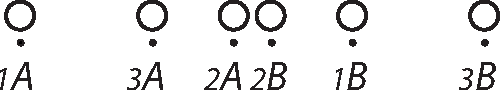
\includegraphics[width=0.36\textwidth]{%
gesamttex/edit_VIII,3/images/LH_35_09_21_005-006_d1_005r.pdf%
}} 
\vspace{0.5em}
\centerline{%
\lbrack\textit{Fig.~1}\rbrack%
}
% \newpage%
\vspace{1em}
%
\pstart\noindent
Cum varii casus circa corporum concursus\protect\index{Sachverzeichnis}{concursus} proponi possint, in quibus nondum omnia sint liquida\lbrack,\rbrack\
%
utile erit eos deligere ante omnia, qui prae caeteris sunt faciliores,%
\protect\index{Sachverzeichnis}{casus facilior concursus} unde paulatim ad caeteros fiat progressus. Tanquam certissimum autem assumo eandem in natura servari 
quantitatem virium,\protect\index{Sachverzeichnis}{quantitas virium}%
\protect\index{Sachverzeichnis}{vis} item eandem servari quantitatem directionis.%
\protect\index{Sachverzeichnis}{quantitas directionis}%
\protect\index{Sachverzeichnis}{directio} 
%
Hinc si duo corpora aequalia et \edtext{similia\protect\index{Sachverzeichnis}{corpora aequalia et similia} concurrant in eadem recta%
\protect\index{Sachverzeichnis}{concursus in eadem recta} generaliter ajo}{\lemma{similia}\Bfootnote{\textit{(1)}~figur \textit{(2)}~concurrant \textit{(a)}~generaliter puto ipsa permutare \textit{(b)}~in eadem recta generaliter \textit{(aa)}~puto \textit{(bb)}~ajo~\textit{L}}}
%
permutari celeritates.%
\protect\index{Sachverzeichnis}{celeritas}%
\protect\index{Sachverzeichnis}{permutatio celeritatum}
\pend
%
\pstart
Ita enim quam minima est mutatio, ita ut priora a \edtext{posteriori\lbrack bu\rbrack s}{\lemma{}\Bfootnote{posterioris \textit{L ändert Hrsg.}}} 
%
discerni non possint. Idem fore arbitror, si corpus quodcunque aequale vel inaequale, mobile vel 
%
\edtext{firmum\lbrack,\rbrack\ modo simplex}{\lemma{firmum}\Bfootnote{\textit{(1)}~inter \textit{(2)}~modo \textit{(a)}~durum seu rigidum inter \textit{(aa)}~duos \textit{(bb)}~duo \textit{(b)}~simplex~\textit{L}}} 
%
aut ex pluribus compositum inter duo corpora 
%
\edtext{sit interjectum,}{\lemma{sit}\Bfootnote{\textit{(1)}~interpositum \textit{(2)}~interjectum,~\textit{L}}} 
%
modo sit rigidum:%
\protect\index{Sachverzeichnis}{corpus inter duo interjectum}%
\protect\index{Sachverzeichnis}{corpus rigidum} ut \pend
%
\vspace{0.5em} %%%%%%%%% Diagramm 2
\centerline{%
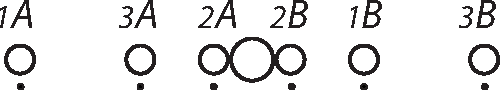
\includegraphics[width=0.36\textwidth]{%
gesamttex/edit_VIII,3/images/LH_35_09_21_005-006_d2_005r.pdf%
}} 
\vspace{0.5em}
\centerline{%
\lbrack\textit{Fig.~2}\rbrack%
}
% \newpage%
\vspace{1em}
%
%
\pstart
Hinc etiam si plures globi in directum positi%
\protect\index{Sachverzeichnis}{globi plures in directum positi} aequales, in alios globos plures in directum positos%
\protect\index{Sachverzeichnis}{globi plures in directum positi} \edtext{ingruant, similis}{\lemma{ingruant,}\Bfootnote{\textit{(1)}~post \textit{(2)}~similis~\textit{L}}} fiet 
%
\edlabel{35_09_21_005-006_1a}%
\edtext{}{{\xxref{35_09_21_005-006_1a}{35_09_21_005-006_1b}}\lemma{permutatio.}%
\Bfootnote{\textit{(1)}~Quodsi plures g \textit{(2)}~Quodsi \textit{(a)}~plures globi inaequales \textit{(b)}~numerus~\textit{L}}}%
permutatio\protect\index{Sachverzeichnis}{permutatio celeritatum}. 
\pend
%
\vspace{1.5em} %%%%%%%%% Diagramm 3
\centerline{%
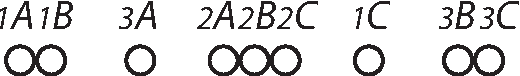
\includegraphics[width=0.38\textwidth]{%
gesamttex/edit_VIII,3/images/LH_35_09_21_005-006_d3_005r.pdf%
}} 
\vspace{0.5em}
\centerline{%
\lbrack\textit{Fig.~3}\rbrack%
}
% \newpage%
\vspace{1em}
%
\pstart  
Quodsi numerus\edlabel{35_09_21_005-006_1b}
%
globorum aequalium concurrentium%
\protect\index{Sachverzeichnis}{globi aequales concurrentes} sit inaequalis\lbrack,\rbrack\ videamus quid sit dicendum? Dico in conflictu\protect\index{Sachverzeichnis}{conflictus} non amplius spectari societatem, aut quae cum quibus venerint, modo possit obtineri permutatio\protect\index{Sachverzeichnis}{permutatio celeritatum}, 
%
ita in apposito casu cum \textit{AB} simul venerint et \textit{C} solum, post \edtext{conflictum\protect\index{Sachverzeichnis}{conflictus} \textit{A} solo relicto}{\lemma{conflictum \textit{A}}\Bfootnote{\textit{(1)}~solum unum relictum \textit{(2)}~solo relicto~\textit{L}}}
\textit{B} se adjungit ad \textit{C}, et cum eo reflexo pergit. \pend
%
\pstart \lbrack5~v\textsuperscript{o}\rbrack\
\edlabel{35_09_21_005-006_3a}%
In obliquis concursibus\protect\index{Sachverzeichnis}{concursus obliquus} manifestum \edtext{est permutationem}{\lemma{est}\Bfootnote{\textit{(1)}~nulla \textit{(2)}~permutationem~\textit{L}}} obtineri non posse, ut omnia sint quemadmodum ante concursum.%
\protect\index{Sachverzeichnis}{concursus} 
\pend
%
\vspace{1.0em} %%%%%%%% Diagramme 4-5
\centerline{%
\hfill
\protect\raisebox{1em}{%
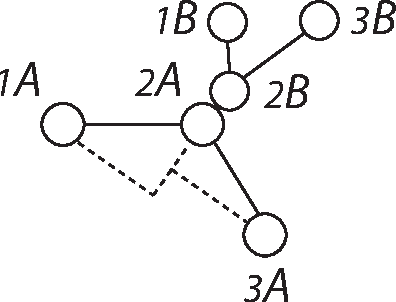
\includegraphics[width=0.23\textwidth]{%
gesamttex/edit_VIII,3/images/LH_35_09_21_005-006_d4_005v.pdf%
}}%
\hfill%
%ggf. eins der Diagramme:    }%
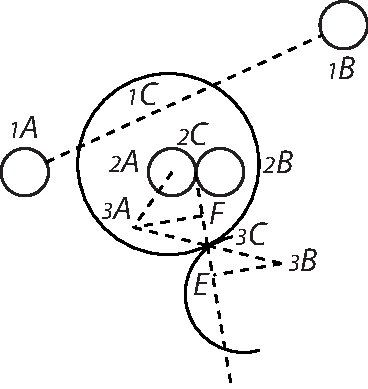
\includegraphics[width=0.26\textwidth]{%
gesamttex/edit_VIII,3/images/LH_35_09_21_005-006_d5_005v.pdf%
}
\hfill%
} % Hier leere Zeile

\vspace{0em}
\centerline{%
\hfill
\lbrack\textit{Fig.~4%
}\rbrack \hspace*{45mm}
\lbrack\textit{Fig.~5, gestr.%
}\rbrack
\hfill%
}
% \newpage%
\vspace{0.5em}
%
%
%%%%%%%%% Diagramm 6
\centerline{%
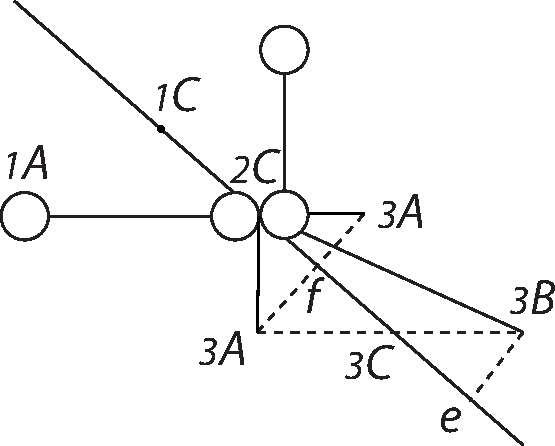
\includegraphics[width=0.3\textwidth]{%
gesamttex/edit_VIII,3/images/LH_35_09_21_005-006_d6_005v.pdf%
}} 
\vspace{0em}
\centerline{%
\astrosun\ \lbrack\textit{Fig.~6}\rbrack%
}
% \newpage%
\vspace{1em}
%
\pstart 
\edtext{}{\lemma{}%	A-Fn zu Fig. 6
\Afootnote{\textit{Am Rand, nachgetragen}: %
ad Fig.~\astrosun\ \lbrack= \textit{Fig.~6}\rbrack \newline %
${\scriptstyle\textit{2}}C{\scriptstyle\textit{3}}C=c, {\scriptstyle\textit{3}}Cf\text{\textsuperscript{\lbrack{}a\rbrack}}={\scriptstyle\textit{3}}Ce\text{\textsuperscript{\lbrack{}a\rbrack}}=m$ \newline %
%
${\scriptstyle\textit{3}}Af={\scriptstyle{3}}Be=n$ \newline %
%
$\overline{{\scriptstyle\textit{2}}C{\scriptstyle\textit{3}}A}^2=c^2-2cm+m^2+n^2$ \newline %
$\lbrack{}\overline{{\scriptstyle\textit{2}}C{\scriptstyle\textit{3}}B}^2\rbrack{}\textsuperscript{\lbrack{}b\rbrack{}}=c^2+2cm+m^2+n^2$ \newline %
\protect\rule[0cm]{0mm}{16pt}$\left. \protect\displaystyle\efrac{{\scriptstyle\textit{1}}A{\scriptstyle\textit{2}}C^2}{{\scriptstyle\textit{1}}B{\scriptstyle\textit{2}}C^2} \right\}%
=(2)c^2+(2)m^2+(2)n^2=vv$ seu $=(2)\overline{{\scriptstyle\textit{2}}C{\scriptstyle\textit{3}}C}^2%
+(2)\overline{{\scriptstyle\textit{3}}\lbrack C\rbrack F}^2\textsuperscript{\lbrack{}c\rbrack{}}%
+(2)\overline{{\scriptstyle\textit{3}}BE}^2$ \newline %
Videamus jam an possit cadere \textit{{\scriptsize3}A} in rectam \textit{{\scriptsize1}A{\scriptsize2}A}, seu angulum %
\textit{{\scriptsize 2}C}\textit{{\scriptsize3}A} ad \textit{{\scriptsize 1}C{\scriptsize 2}C} esse datum, seu dari rationem %
$\sqrt{c^2-2cm+m^2+n^2}$ ad $c-m$, seu rationem \textit{n} ad \textit{m} unde patet progredi \textit{A} %
trans \textit{{\scriptsize2}A} quod videndum an possibile. \newline\newline %
{\footnotesize % Marginalienapparat
\textsuperscript{\lbrack{}a\rbrack{}} \textit{e}, \textit{f}: Leibniz verwendet für die Punkte \textit{e} und \textit{f} große wie kleine Buchstaben. \quad %
\textsuperscript{\lbrack{}b\rbrack{}} \textit{{\scriptsize 2}C{\scriptsize3}B} \textit{L ändert Hrsg.} \quad %
\textsuperscript{\lbrack{}c\rbrack{}} $(2)\overline{{\scriptstyle\textit{3}}AF}^2$ \textit{L ändert Hrsg.}%
}}}%
%
Examinare etiam operae pretium est quid fiat si corpus unum incurrat in alterum, sic ut et alterum moveatur lineaeque motus%
\protect\index{Sachverzeichnis}{linea motus} sint obliquae; 
%
et tamen, vicissim alterum non incurreret ipsi, incurrit enim quod ab altero etiam quiescente impeditur, fieri enim potest, ut \textit{A} 
%
incurrat in \textit{B}, at \textit{B} tantum raderet \textit{A}, si quiesceret. Videndum est an hoc casu non tantum ipsius \textit{B}, sed et 
%
ipsius \textit{A} %
linea directionis\protect\index{Sachverzeichnis}{linea directionis} a priore divergat. Quaeramus rem ex generalibus principiis servatae quantitatis motus,\protect\index{Sachverzeichnis}{quantitas motus}%
\protect\index{Sachverzeichnis}{principium servatae quantitatis motus} et servati centri 
%
gravitatis.\protect\index{Sachverzeichnis}{centrum gravitatis}%
\protect\index{Sachverzeichnis}{principium servati centri gravitatis} 
%
Habemus loca \textit{{\scriptsize 1}C.{\scriptsize 2}C.{\scriptsize 3}C}. 
%
Quaeritur unum adhuc ut \textit{{\scriptsize3}B}, quo dato statim habebitur et \textit{{\scriptsize3}A}, 
%
jungendo \textit{{\scriptsize3}B{\scriptsize 3}C} et producendo in ${\scriptstyle\textit{3}\,}C{\scriptstyle\textit{3}}A = 
%
{\scriptstyle\textit{3}\,}C{\scriptstyle\textit{3}}B$. Sumto ergo \textit{{\scriptsize3}B} pro arbitrio, unde in productam
%
 \textit{{\scriptsize 1}C{\scriptsize 3}C} ducatur perpendicularis \textit{{\scriptsize 3}BE}, et jungatur 
%
\textit{{\scriptsize2}B{\scriptsize3}B}, id est 
%
\edtext{\textit{{\scriptsize2}B{\scriptsize3}}\lbrack\textit{C}\rbrack\lbrack,\rbrack}{%
\lemma{}%
\Bfootnote{%
\textit{{\scriptsize2}B{\scriptsize3}B} %
\textit{L ändert Hrsg.}}}
%
habeo enim \textit{A} et \textit{B} quasi pro punctis. Similiter, sit ex \textit{{\scriptsize3}A} in \textit{CC} perpendicularis 
%
\edtext{\textit{{\scriptsize 3}AF}, et jungatur}{\lemma{}\Bfootnote{\textit{{\scriptsize 3}AF}, et \textbar\ et \textit{streicht Hrsg.} \textbar\ jungatur~\textit{L}}} 
%
\textit{{\scriptsize3}A{\scriptsize3}A} 
%
\edtext{seu \textit{{\scriptsize 2}C}\textit{{\scriptsize3}A},}{\lemma{}\Bfootnote{seu \textit{{\scriptsize 2}C}\textit{{\scriptsize3}A} \textit{erg.~L}}}
%
debet (ob corpora \textit{A} et \textit{B} aequalia) $\overline{\text{\textit{\scriptsize 2}}A\text{\textit{\scriptsize 3}}A}^2 + \overline{\text{\textit{\scriptsize 2}}B\text{\textit{\scriptsize 3}}B}^2,$ esse aequalia
%
 $\overline{\text{\textit{\scriptsize 1}}A\text{\textit{\scriptsize 2}}A}^2 + \overline{\text{\textit{\scriptsize 1}}B\text{\textit{\scriptsize 2}}B}^2$. 
%
Sunt autem \textit{{\scriptsize2}A{\scriptsize3}A} et \textit{{\scriptsize1}B{\scriptsize2}B} 
%
\edtext{aequales.\edlabel{35_09_21_005-006_3b} Cum}{\lemma{aequales.}\Bfootnote{\textit{(1)}~Problema igitur sic apte solvetur: fiat triangulum rectangulum \textit{LMN}, %
\protect\raisebox{-0.2em}{\protect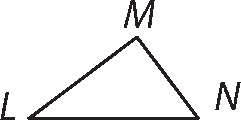
\includegraphics[width=0.12\textwidth]{gesamttex/edit_VIII,3/images/LH_35_09_21_005-006_d7_005v.pdf}}~%Diagramm 7
\lbrack\textit{Fig.~7}\rbrack %
\quad\textit{(a)}~eritque \textit{(b)}~ita ut sit \textit{LN} sit aequ. \textit{{\scriptsize1}A{\scriptsize 2}C}, et \textit{(2)}~Cum~\textit{L}}} 
%
autem hoc modo calculandi corpora ut puncta considerando,%
\protect\index{Sachverzeichnis}{consideratio corporis ut punctum} perinde sit ac si utrinque sit concursus\protect\index{Sachverzeichnis}{concursus}, an vero ab altera parte tantum rasio,%
\protect\index{Sachverzeichnis}{rasio} et licet corpora deinde substituamus tamen quia 
%
\edtext{regula servatae}{\lemma{regula}\Bfootnote{\textit{(1)}~servatura \textit{(2)}~servatae~\textit{L}}}
in summa directionis%
\protect\index{Sachverzeichnis}{directio}%
\protect\index{Sachverzeichnis}{regula in summa servatae directionis} 
%
non multum abludit, manifestum est etiam corpus quod radi tantum videtur\lbrack,\rbrack\ simul abripi, quia revera compressione%
\protect\index{Sachverzeichnis}{compressio}
%
\lbrack6~r\textsuperscript{o}\rbrack\ 
%
fit, ut non tantum radat, sed et in alterum subingrediatur, unde 
%
\edtext{utique confirmatur omnia}{\lemma{utique}\Bfootnote{\textit{(1)}~ex resu \textit{(2)}~confirmatur \textit{(a)}~dura \textit{(b)}~omnia~\textit{L}}}
%
rigida%
\protect\index{Sachverzeichnis}{corpus rigidum} debere flexilia%
\protect\index{Sachverzeichnis}{corpus flexile} esse licet 
%
\edlabel{35_09_21_005-006_2a}%
\edtext{}{{\xxref{35_09_21_005-006_2a}{35_09_21_005-006_2b}}\lemma{insensibiliter.}\Bfootnote{\textit{(1)}~Si plura  \textbar\ duobus \textit{erg.} \textbar\ conjungantur corpora aequalia duae regulae nostrae ad determinandum non sufficiunt \textit{(2)}~Sed hinc~\textit{L}}}%
insensibiliter. 
%
\pend \pstart 
Sed hinc\edlabel{35_09_21_005-006_2b}
%
consideranti tamen \edtext{dubium occurrit}{\lemma{dubium}\Bfootnote{\textit{(1)}~incurrit \textit{(2)}~occurrit~\textit{L}}}, an non %
consideratio corporis ut punctum\protect\index{Sachverzeichnis}{consideratio corporis ut punctum} nimis \edtext{recedat aut}{\lemma{recedat}\Bfootnote{\textit{(1)}~nam revera si \textit{(2)}~aut~\textit{L}}} an non regula illa hoc modo evertatur, de linea 
%
\edtext{impressionis\protect\index{Sachverzeichnis}{linea impressionis} in}{%
\lemma{impressionis}%
\Bfootnote{%
\textit{(1)}~semper sumen %
\textit{(2)}~in~\textit{L}}}
%
ictu\protect\index{Sachverzeichnis}{ictus} semper sumenda in perpendiculari. Nam hoc posito videtur necessario in casu rasionis\protect\index{Sachverzeichnis}{rasio} linea reflexionis\protect\index{Sachverzeichnis}{linea reflexionis} ipsius \textit{A} esse ipsa linea incursionis\protect\index{Sachverzeichnis}{linea incursionis}, nam si incursum\protect\index{Sachverzeichnis}{incursus} ipsius \textit{B} in \textit{A} pro rasione\protect\index{Sachverzeichnis}{rasio} sumamus utcunque exiguum, id propemodum fiet. Haec igitur faciunt, 
%
\edtext{ut illa}{\lemma{ut}\Bfootnote{\textit{(1)}~linea \textit{(2)}~illa~\textit{L}}}
%
regula in dubium revocanda 
%
\edtext{videatur.}{\lemma{}%	A-Fn. zwischen den Absätzen
\Afootnote{\textit{Am Ende des Absatzes zwischen den Zeilen}: %
Imo jam video naturam rei prospexisse, et haec minime pugnare, ideo enim per sola puncta determinari non potest motus.}} 
\pend 
\pstart 
Si plura sint 
%
\edtext{corpora quae}{%
\lemma{corpora}%
\Bfootnote{%
\textit{(1)}~, licebit ne %
\textit{(2)}~quae~\textit{L}%
}}
%
concurrant, licebitne problemata ita solvere, 
%
\edtext{ut in singulis}{\lemma{ut}\Bfootnote{\textit{(1)}~si \textit{(2)}~in singulis singula serv \textit{(3)}~in singulis~\textit{L}}} 
%
paribus quam maxime licet eadem servetur quantitas virium\protect\index{Sachverzeichnis}{quantitas virium} et linea 
%
\edtext{directionum\protect\index{Sachverzeichnis}{linea directionum}, et annon}{\lemma{directionum,}\Bfootnote{\textit{(1)}~quod cum \textit{(a)}~liceat \textit{(b)}~non liceat \textit{(2)}~et annon~\textit{L}}} 
%
plus favendum sit uni pari quam alteri videndum est et in summa dispiciendum quomodo res possit dirigi, ut omnia quoad licet sint prioribus similia. Videamus quomodo ex principio similitudinis\protect\index{Sachverzeichnis}{principium similitudinis} demonstremus quae ex duobus aliis demonstravimus\lbrack,\rbrack\ ex principio servandae potentiae\protect\index{Sachverzeichnis}{principium servandae potentiae} et 
%
\edtext{directionis,\protect\index{Sachverzeichnis}{principium servandae directionis} etiam}{\lemma{directionis,}\Bfootnote{\textit{(1)}~ut possumus \textit{(2)}~etiam~\textit{L}}} 
%
pro duobus inaequalibus;%
\protect\index{Sachverzeichnis}{corpora duo inaequalia} ut principium quoque similitudinis\protect\index{Sachverzeichnis}{principium similitudinis} ad plura propagemus. 
%
\pend \pstart 
%
Multum ergo adhuc absumus a perfectione. Videtur tamen utique ratio habenda superficiei excipientis,%
\protect\index{Sachverzeichnis}{superficies corporis excipientis} non 
%
\edtext{solum potentiarum%
\protect\index{Sachverzeichnis}{potentia}}{\lemma{solum}\Bfootnote{\textit{(1)}~magnitudinis \textit{(2)}~potentiarum~\textit{L}}}
%
\lbrack6~v\textsuperscript{o}\rbrack\ et centrorum.%
\protect\index{Sachverzeichnis}{centrum gravitatis} Quamdiu tamen punctis  
tantum pro corporibus utimur, minus turbant. 
%
\pend
%
\vspace{2.0em} %%%%%%%%% Diagramm 8
\centerline{%
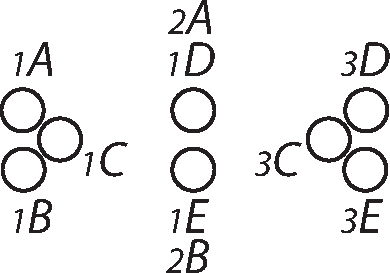
\includegraphics[width=0.25\textwidth]{%
gesamttex/edit_VIII,3/images/LH_35_09_21_005-006_d8_006v.pdf%
}} 
\vspace{0.5em}
\centerline{%
\lbrack\textit{Fig.~8}\rbrack%
}
% \newpage%
\vspace{1.5em}
%
\pstart
Si \textit{{\scriptsize1}A{\scriptsize1}B{\scriptsize 1}C} incurrat in \textit{{\scriptsize 1}D{\scriptsize 1}E} \edtext{quiescentia}{\lemma{}\Bfootnote{quiescentia \textit{erg.~L}}}, videtur \textit{{\scriptsize2}A} et \textit{{\scriptsize2}B} succedere in locum
\textit{{\scriptsize 1}D{\scriptsize 1}E}, et \textit{CDE} simul ire, ita enim omnia fiunt, ac si nullus 
%
\edtext{fuisset incursus\protect\index{Sachverzeichnis}{incursus}, at hoc}{\lemma{fuisset}\Bfootnote{\textit{(1)}~mutatio \textit{(2)}~incursus, \textit{(a)}~sed  \textit{(b)}~hinc  \textit{(c)}~at hoc~\textit{L}}}
%
tamen non videtur locum habere posse sed potius \textit{D} et \textit{E} procedere in linea per centra \textit{{\scriptsize 2}C} et \textit{{\scriptsize 1}C} transeunte.%
\protect\index{Sachverzeichnis}{linea per centra transiens} Similesque fingi possunt casus, ne scilicet nimium tribuamus primis illis congruentiis%
\protect\index{Sachverzeichnis}{congruentia} quae in simplicioribus casibus%
\protect\index{Sachverzeichnis}{casus simplicior concursus} observantur. \pend
%
\pstart 
Videndum et variis modis quid fiat \edtext{si corpora}{\lemma{si}\Bfootnote{\textit{(1)}~corpus \textit{(2)}~corpora~\textit{L}}} duo mobilia%
\protect\index{Sachverzeichnis}{corpus mobile} per unum immobile%
\protect\index{Sachverzeichnis}{corpus immobile} inter se communicent, et inprimis si incursus in immobile sint obliqui\protect\index{Sachverzeichnis}{incursus obliquus}, quae quidem omnia ex solis duobus principiis nostris poterunt determinari. Ex iisdem etiam determinari potest, quid fiat si plura duobus corpora assumantur, v.g.\ tria, sed ita ut duo ex illis tractari debeant eodem modo ut in proximo exemplo \textit{A} et \textit{B}, item \textit{D} et \textit{E}. Imo fieri potest ut tria, vel quatuor tractari debeant eodem modo, quibus casibus semper solutio habetur. 
\pend
\count\Afootins=1200%
\count\Bfootins=1200%
\count\Cfootins=1200